\documentclass[12pt,a4paper]{article}

\usepackage{hyperref}
\usepackage{graphicx, epstopdf} % eps... for e.g. MATLAB-Grafiken im .eps-format
\graphicspath{{./img/}} % default folder for images
\usepackage{float}
\usepackage{xcolor}
\usepackage{amsmath, amsfonts, amssymb, amsthm} % enhanced math writing
\let\vec\mathbf % vektoren bold und nicht arrow
\setlength{\parindent}{0em} % keine Einrueckungen, sonst \noindent

\usepackage[tmargin=1in,bmargin=1in,lmargin=1.25in,rmargin=1.25in]{geometry} % MSWord-Format

% customize Header and Footer
\usepackage{fancyhdr, lastpage}
\pagestyle{fancy}
\fancyhf{}
\lhead{MAWE - DFT Matrix Dokumentation}
\rhead{Jonas Berger, Ahmed Ibrahim}
\lfoot{\today}
\rfoot{Seite \thepage \space von \pageref{LastPage}}
\renewcommand{\headrulewidth}{0.4pt}
\renewcommand{\footrulewidth}{0.4pt}

% Umlaute-Encoding und Standardschrift einstellen
\usepackage[ngerman]{babel}
\usepackage[utf8]{inputenc}
\usepackage[T1]{fontenc}
\usepackage{lmodern}

\usepackage{listings, lstautogobble} % adding code listing support
\newcommand*\listingspath[1]{\lstset{inputpath=#1}}
\listingspath{../matlab_workspace/} % default folder for codes

% complete table of contents
\usepackage[nottoc,numbib]{tocbibind}
\renewcommand{\lstlistoflistings}{\begingroup
	\tocfile{\lstlistlistingname}{lol}
\endgroup}

%\renewcommand{\contentsname}{Inhaltsverzeichnis}
\renewcommand{\lstlistlistingname}{Codelisting}
%\renewcommand{\listfigurename}{Abbildungsverzeichnis}
%\renewcommand{\listtablename}{Tabellenverzeichnis}

\usepackage{matlab-prettifier}

\usepackage{accsupp}
\newcommand{\noncopynumber}[1]{%
	\BeginAccSupp{method=escape,ActualText={}}%
	#1%
	\EndAccSupp{}%
}

% globale Code-Settings
\lstset{
	style=Matlab-editor,
	basicstyle=\scriptsize,
	captionpos = b,
	frame = single,
	numbers = left,
	numberstyle=\tiny\noncopynumber,
	literate=
	{á}{{\'a}}1 {é}{{\'e}}1 {í}{{\'i}}1 {ó}{{\'o}}1 {ú}{{\'u}}1
	{Á}{{\'A}}1 {É}{{\'E}}1 {Í}{{\'I}}1 {Ó}{{\'O}}1 {Ú}{{\'U}}1
	{à}{{\`a}}1 {è}{{\`e}}1 {ì}{{\`i}}1 {ò}{{\`o}}1 {ù}{{\`u}}1
	{À}{{\`A}}1 {È}{{\'E}}1 {Ì}{{\`I}}1 {Ò}{{\`O}}1 {Ù}{{\`U}}1
	{ä}{{\"a}}1 {ë}{{\"e}}1 {ï}{{\"i}}1 {ö}{{\"o}}1 {ü}{{\"u}}1
	{Ä}{{\"A}}1 {Ë}{{\"E}}1 {Ï}{{\"I}}1 {Ö}{{\"O}}1 {Ü}{{\"U}}1
	{â}{{\^a}}1 {ê}{{\^e}}1 {î}{{\^i}}1 {ô}{{\^o}}1 {û}{{\^u}}1
	{Â}{{\^A}}1 {Ê}{{\^E}}1 {Î}{{\^I}}1 {Ô}{{\^O}}1 {Û}{{\^U}}1
	{ã}{{\~a}}1 {ẽ}{{\~e}}1 {ĩ}{{\~i}}1 {õ}{{\~o}}1 {ũ}{{\~u}}1
	{Ã}{{\~A}}1 {Ẽ}{{\~E}}1 {Ĩ}{{\~I}}1 {Õ}{{\~O}}1 {Ũ}{{\~U}}1
	{œ}{{\oe}}1 {Œ}{{\OE}}1 {æ}{{\ae}}1 {Æ}{{\AE}}1 {ß}{{\ss}}1
	{ű}{{\H{u}}}1 {Ű}{{\H{U}}}1 {ő}{{\H{o}}}1 {Ő}{{\H{O}}}1
	{ç}{{\c c}}1 {Ç}{{\c C}}1 {ø}{{\o}}1 {å}{{\r a}}1 {Å}{{\r A}}1
	{€}{{\euro}}1 {£}{{\pounds}}1 {«}{{\guillemotleft}}1
	{»}{{\guillemotright}}1 {ñ}{{\~n}}1 {Ñ}{{\~N}}1 {¿}{{?`}}1 {¡}{{!`}}1,
	autogobble=true            % autoalign text
}

\title{DFT Matrix Dokumentation}
\author{Jonas Berger, Ahmed Ibrahim}
\date{\today}

\begin{document}
	\maketitle
	\thispagestyle{empty}
	\pagebreak
	\tableofcontents
	\pagebreak
	
	\section{Theorie}
	Mithilfe der diskreten Fourier Transformation (DFT) kann der Frequenzgehalt eines zeit-diskreten Signals berechnet werden.
	Dadurch ist diese Transformation das Äquivalent zur Fourier Transformation (FT) für zeit-kontinuierliche Signale.\\\\
	Das Kernstück der DFT ist die DFT-Matrix $W$, die multipliziert mit dem diskreten Zeitvektor $x$ den Frequenzvektor $X$ ergibt.
	\begin{equation*}
		X = W \cdot x
	\end{equation*}	
	Dabei wird die DFT-Matrix $W$ aus folgenden Basisvektoren aufgebaut:
	\begin{equation*}
		\vec{u}_0=\begin{pmatrix} 1 \\ 1 \\ \vdots \\ 1 \end{pmatrix},
		\vec{u}_1=\begin{pmatrix} 1 \\ e^{i\frac{2\pi}{N}1\cdot 1} \\ \vdots \\ e^{i\frac{2\pi}{N}1\cdot (N-1)} \end{pmatrix},
		\vec{u}_2=\begin{pmatrix} 1 \\ e^{i\frac{2\pi}{N}2\cdot 1} \\ \vdots \\ e^{i\frac{2\pi}{N}2\cdot (N-1)} \end{pmatrix}, \cdots, 
		\vec{u}_{N-1}=\begin{pmatrix} 1 \\ e^{i\frac{2\pi}{N}(N-1)\cdot 1} \\ \vdots \\ e^{i\frac{2\pi}{N}(N-1)\cdot (N-1)} \end{pmatrix}
	\end{equation*}
	Daraus ergibt sich folgende Formel zur Berechnung der einzelnen Frequenzkomponenten $X_k$
	\begin{equation*}
		X_k = \langle \vec{u}_k,\vec{x} \rangle = \sum_{k=0}^{N-1} e^{-i\frac{2\pi}{N}k\cdot l} x_l
		\quad
		\text{wobei} \; W = e^{-i\frac{2\pi}{N}k\cdot l}
	\end{equation*}
	Analog zur DFT gibt es auch die inverse DFT (IDFT) zur Berechnung der einzelnen Zeitkomponenten $x_l$:
	\begin{equation*}
		x_l = \frac{1}{N}\sum_{k=0}^{N-1} e^{i\frac{2\pi}{N}k\cdot l} X_k \quad
		\text{wobei} \; W^{-1} = \frac{1}{N}e^{i\frac{2\pi}{N}k\cdot l}
	\end{equation*}
	
	\pagebreak
	
	\section{Ermittlung einer DFT-Matrix mit unterschiedlichen Methoden}
	\label{sec:dftmat}
	Es sollen in MATLAB Funktionen geschrieben werden, die jeweils eine DFT-Matrix mit der Gr\"o{\ss}e NxN ermitteln. Implementiert wird jede Funktion unter Verwerwendung von unterschiedlichen Methoden.
	
	\subsection{Methode mit doppelter for-Schleife}
	Im nachfolgenden Code-Ausschnitt ist die Implementierung mit doppelter for-Schleife ersichtlich: \\
	%\begin{minipage}{\textwidth}
	\lstinputlisting[caption={Code-Implementierung mit doppelter for-Schleife}, label = {lst:dftmatrix1}, firstline=1, lastline=19]{dftmatrix1.m}
	%\end{minipage}

	\subsection{Methode mit Exponenzieren}
	Im nachfolgenden Code-Ausschnitt ist die Implementierung mit elementweisem Exponenzieren ersichtlich: \\
	\lstinputlisting[caption={Code-Implementierung mit Exponenzieren}, label = {lst:dftmatrix2}, firstline=1, lastline=15]{dftmatrix2.m}
	
	\pagebreak

	\subsection{Methode mit elementweisem Potenzieren}
	Im nachfolgenden Code-Ausschnitt ist die Implementierung mit elementweisem Potenzieren ersichtlich: \\
	\lstinputlisting[caption={Code-Implementierung mit elementweisem Potenzieren}, label = {lst:dftmatrix3}, firstline=1, lastline=17]{dftmatrix3.m}
	
	\subsection{Verwendung der Vandermonde-Matrix}
	Im nachfolgenden Code-Ausschnitt ist die Implementierung mittels Vandermonde-Matrix ersichtlich: \\
	\lstinputlisting[caption={Code-Implementierung mittels Vandermonde-Matrix}, label = {lst:dftmatrix4}, firstline=1, lastline=19]{dftmatrix4.m}
	
	\pagebreak

	\subsection{Verwendung der Fast Fourier Transformation (FFT)}
	Im nachfolgenden Code-Ausschnitt ist die Implementierung mit der Fast Fourier Transformation (kurz FFT) ersichtlich: \\
	\lstinputlisting[caption={Code-Implementierung mit Fast Fourier Transformation}, label = {lst:dftmatrix5}, firstline=1, lastline=12]{dftmatrix5.m}
		
	\pagebreak
	
	\section{Ermittlung der Rechenzeiten der unterschiedlichen Methoden zur Erstellung einer DFT-Matrix}
	Es sollen nun alle, in Abschnitt \ref{sec:dftmat}, implementierten Funktionen miteinander im Bezug auf die Rechenzeit miteinander verglichen werden. 
	Dazu soll ein MATLAB-Skript geschrieben werden, sodass jede individuelle Funktion eine DFT-Matrix von $N=1$ bis $N=2^{8}=256$ berechnet. Dabei wird mit tic und toc die Zeitdauer jeder einzelner Funktions-Ausführung gemessen.
	Dabei wird jede Messung 5-mal ausgef\"uhrt und der Mittelwert der ermittelten Zeit gebildet, um etwaige Schwankungen auszugleichen.
	Abschlie{\ss}end soll die Rechenzeit in Abh\"angikeit der Größe $N$ der Matrix, jeder Funktion, in Form einer Grafik gegen\"ubergestellt werden.
	
	\subsection{Code-Implementierung}
	\label{sec:rechzeitimpl}
	\lstinputlisting[caption={Code-Implementierung zur Rechenzeitberechnung}, label = {lst:rechencode1}, firstline=1, lastline=127]{dftmatrixvergleich.m}
	
	\subsection{Grafische Gegenüberstellung der Rechenzeiten}
	Die Ausführung des Codes in Abschnitt \ref{sec:rechzeitimpl} resultiert in folgender Grafik:
	
	\begin{figure}[H]
		\centering
		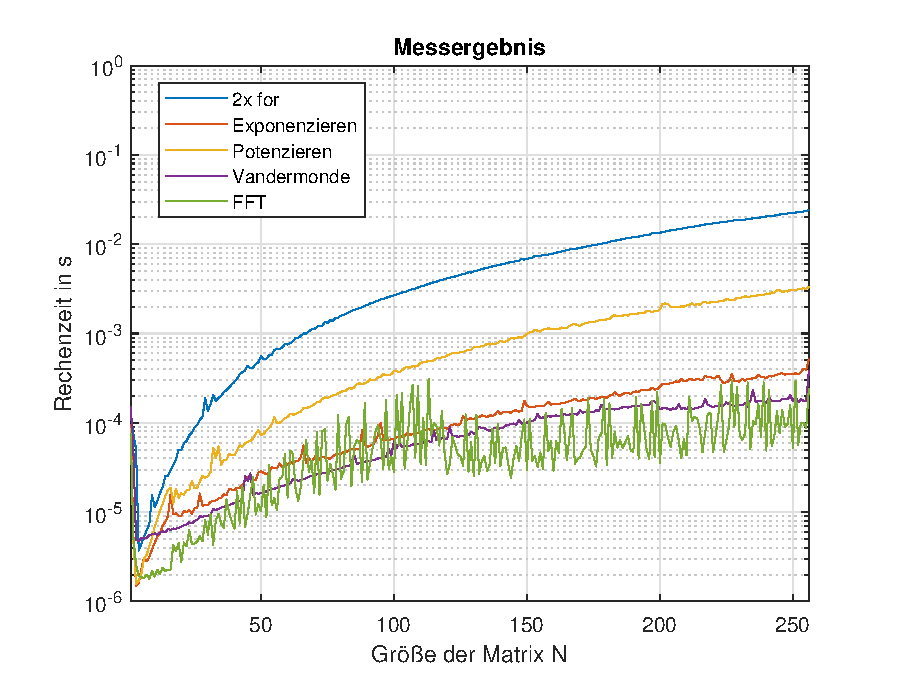
\includegraphics[width=0.9\linewidth]{messergebnis_rechenzeit}
		\caption{Gegenüberstellung der Rechenzeiten}
		\label{fig:messrech}
	\end{figure}

	\underline{Erkenntnis:} Es ist deutlich zu erkennen, dass die Methode mit den doppelten for-Schleifen die langsamste Methode zur Ermittlung einer DFT-Matrix ist. Die schnellste Rechenzeit erreicht die Fast Fourier Transformation, wobei hier trotz der Mittelwertbildung eine große Schwankung der Rechenzeiten erkennbar ist. Die Methode mit der Verwendung der Vandermonde Matrix liegt zwar knapp hinter der FFT, weist aber durchgängig einen praktisch konstanten Verlauf der Rechenzeit auf.

	\pagebreak

	\section{Visualisierung der Basisvektoren im Einheitskreis}
	Die Diskrete Fourier Transformation baut auf die Basisvektoren uk auf. 
	Diese sollen nun grafisch dargestellt werden. Hierfür werden drei Darstellungsformen gewählt: Vektoren im Einheitskreis, Punkte im Einheitskreis und Verlauf im 3-dimensionalen Raum.
	
%	\subsection{Code-Implementierung}
%	\label{sec:basiscode}
%	Nachfolgend die Code-Implementierung:\\
%	\lstinputlisting[caption={Code-Implementierung der Darstellung der Basisvektoren uk}, label = {lst:basisvcode}, firstline=1, lastline=46]{koeffeinheitskreis.m}
	
%	\pagebreak
	
	\subsection{Grafische Darstellungen der Basisvektoren uk}
	Es folgen nun die grafischen Abbildungen der Basisvektoren uk, die mittels MATLAB erzeugt werden.
	\begin{figure}[H]
		\centering
		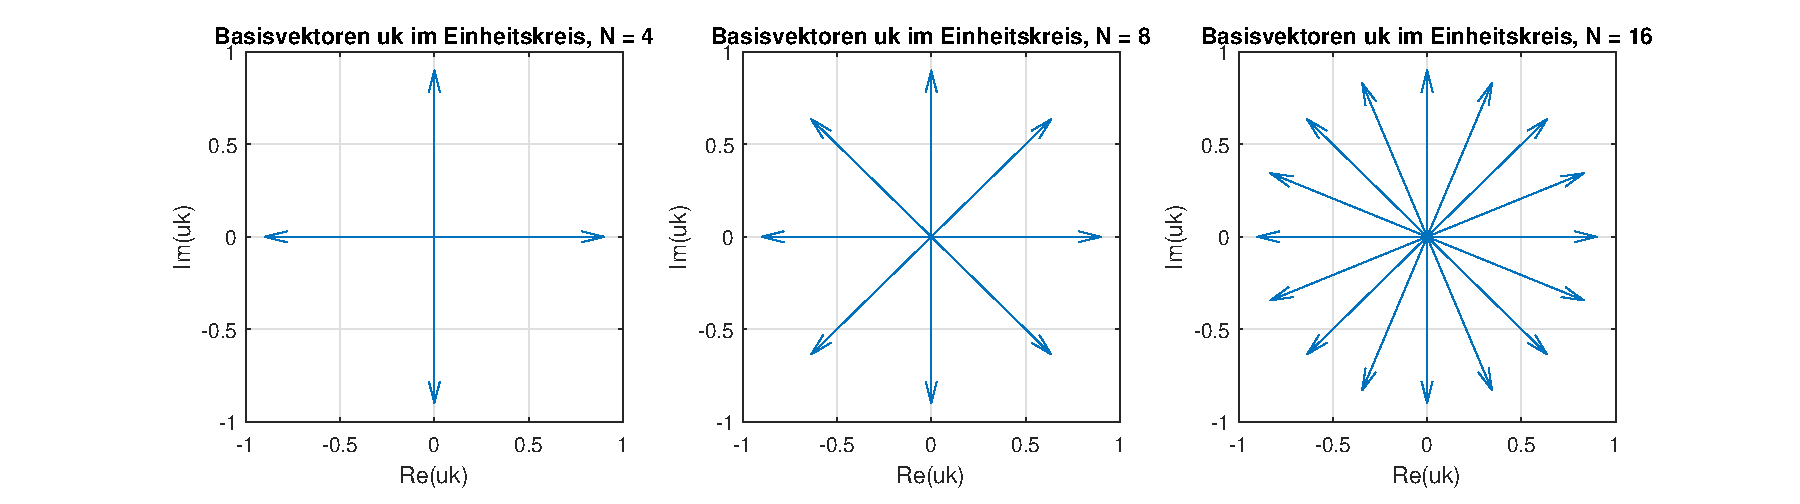
\includegraphics[width=1\linewidth]{basis_vec_Nvar}
		\caption{Vektoren im Einheitskreis}
		\label{fig:bv}
	\end{figure}
	\begin{figure}[H]
		\centering
		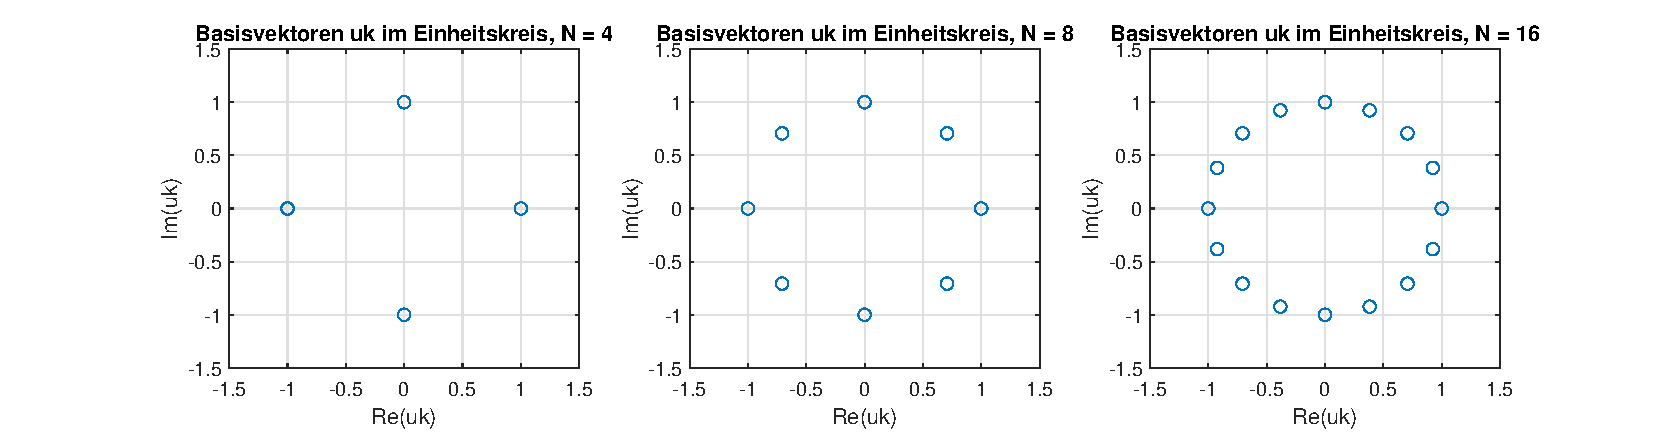
\includegraphics[width=1\linewidth]{basis_punkt_Nvar}
		\caption{Punkte im Einheitskreis}
		\label{fig:bp}
	\end{figure}
	\begin{figure}[H]
		\centering
		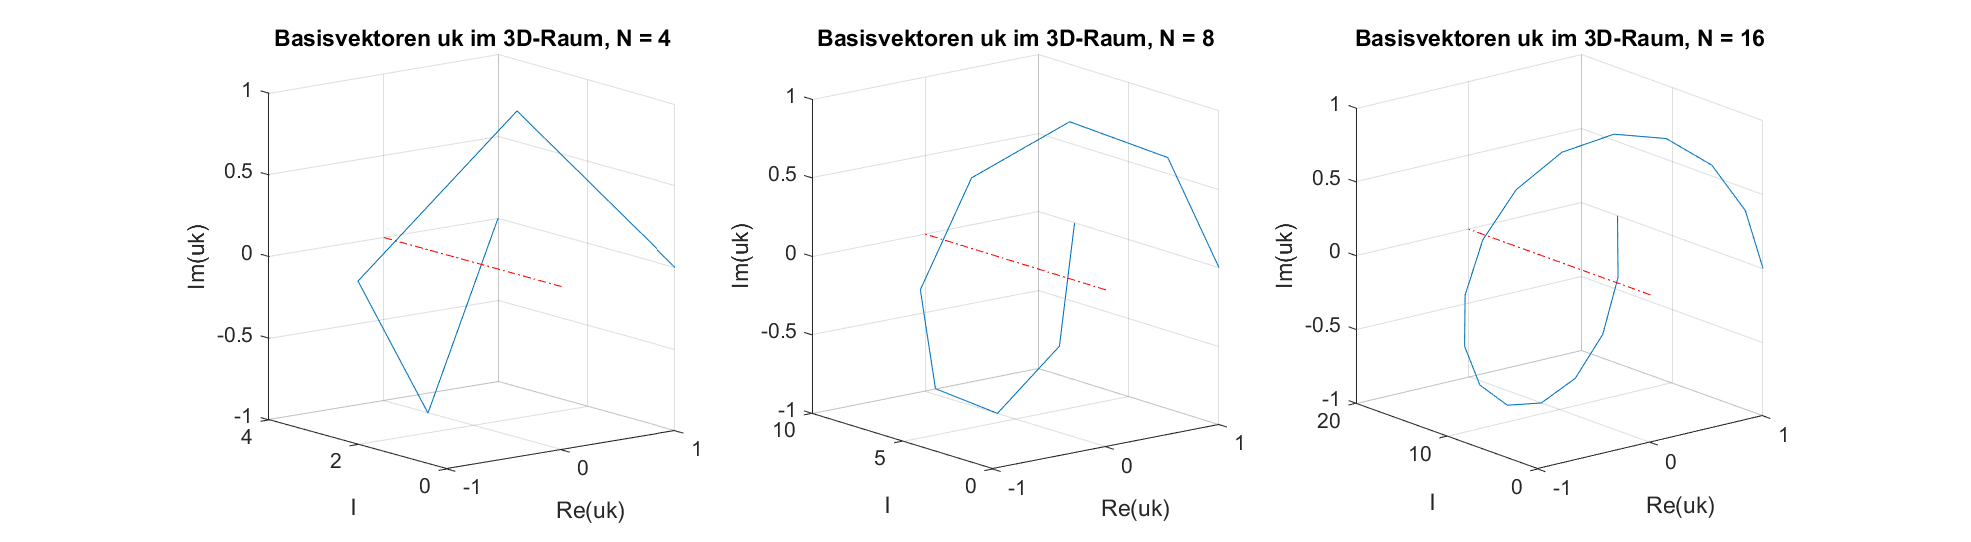
\includegraphics[width=1\linewidth]{basis_3d_Nvar}
		\caption{Verlauf im 3-dimensionalen Raum}
		\label{fig:bd}
	\end{figure}
	
	\pagebreak
	
	\lstlistoflistings
	\listoffigures

\end{document}